\documentclass[11pt, letterpaper]{article}
\setcounter{tocdepth}{4}
\setcounter{secnumdepth}{4}
\usepackage[english]{babel}
\usepackage{fontspec}
\setmainfont{Times New Roman}
\usepackage{float}
\usepackage{tabularx}
\usepackage{adjustbox}
\usepackage{multirow}
\usepackage{longtable}
\usepackage{graphicx}
\usepackage{geometry}
\usepackage{xcolor,colortbl}
\usepackage{sectsty}
\usepackage{titlesec}
\usepackage{textcomp}
\usepackage{subfigure}

\titleformat{\paragraph}
    {\normalfont\normalsize\bfseries}{\theparagraph}{0.2em}{}
\titlespacing*{\paragraph}{\parindent}{1.25ex }{1.75ex}

\sectionfont{\fontsize{18}{15}\selectfont}
\subsectionfont{\fontsize{16}{15}\selectfont}
\subsubsectionfont{\fontsize{14}{15}\selectfont}

\usepackage{enumitem}
\newlist{NH}{enumerate}{1}
\setlist[NH]{label=H\arabic*:}

\newlist{MN}{enumerate}{1}
\setlist[MN]{label=MN\arabic*:}

\newlist{MC}{enumerate}{1}
\setlist[MC]{label=MC\arabic*:}

\newlist{MP}{enumerate}{1}
\setlist[MP]{label=MP\arabic*:}

\usepackage{hyperref}
 \geometry{
    a4paper,
    total={170mm,257mm},
    left=20mm,
    top=25mm,
 }
 \hypersetup{
    colorlinks=true,
    linkcolor=black,
    filecolor=magenta,      
    urlcolor=blue,
}

\usepackage{fancyhdr}
\setlength{\headheight}{27.72354pt}
\addtolength{\topmargin}{-15.72354pt}
\pagestyle{fancy}
\usepackage{tikz}
\usetikzlibrary{automata, positioning, arrows}

\definecolor{maroon}{cmyk}{1,0,1,0.6}

\begin{document}

    \begin{titlepage}
        \begin{center}
        \vspace*{1cm}
            \begin{figure}
                \centering
                
\includegraphics[width=10cm]{images/logos/Logo_Politecnico_Milano.png}
            \end{figure}
            
            \huge
            \textbf{Implementation Specification}

            \vspace{1cm}
        
            \Large
            \textbf{Hypermedia Applications}

            \vspace{1.5cm}

            \begin{figure}[H]
                \centering
                
\includegraphics[width=9cm]{images/logos/i3lab.png}
            \end{figure}

            \vspace{2cm}

            \begin{tabular}{c|c}
                Student & Person Code\\
                \hline\hline
                Davide Di Marco & 10667065\\
                Stefano Fossati & 10569836\\
                Davide Maffi & 10630074\\
                Marco Romanini & 10613151
            \end{tabular}
            \large
            
        \end{center}
    \end{titlepage}

\cleardoublepage

\fancyhead{}
\fancyfoot{}
\fancyhead[L]{Implementation Specification}
\fancyhead[C]{}
\fancyhead[R]{Di Marco, Fossati, Maffi, Romanini}
\cfoot{\thepage}

\tableofcontents
\cleardoublepage
            
\section{Abstract}
This design report is about the Webapp of StartMeUp, a hypothetical venture capital. All of the company's information are available on the website, along with a mechanism to get in touch with them if you want to collaborate or suggest a new project for them to take on.
Information about the firm is provided in the areas of investment, portfolio projects, and staff.
The website's objective is to take the user on a delightful tour through the business and its guiding principles.\\

\section{Teamwork}
\subsection{Components creation}
The work is divided into 4 principal parts associated to each group member but we didn't work in a compartmentalized way.
Once one person had found a nice way to solve an implementation problem, the solution was shared with the others in order to have consistent code.
The aforementioned 4 parts and each respective person are in the Table \ref{tab:parts}.
\vspace{3mm}

\begin{table}[h!]
    \centering
    \begin{tabular}{|c|c|}
        \hline
        All Areas and Area pages, Header and Footer & Davide Di Marco \\
        \hline
        All Projects and Project pages, Database & Stefano Fossati \\
        \hline
        Homepage, Team and Person pages, Animations & Davide Maffi \\
        \hline
        About Us and Contact Us pages, Forms handling & Marco Romanini \\
        \hline
    \end{tabular}
    \caption{Parts of the website associated to each team member}
    \label{tab:parts}
\end{table}

\noindent 
\subsection{Work division}
The StartMeUp webiste can be found \href{https://hypermedia-website.vercel.app/}{here} and we also structured a \href{https://github.com/stefanofossati/hypermedia-website} {Github repository} in order to parallelize the work on the different parts being consistent with the standard way of managing a team work.
First we locked the \emph{main} in order to not push there until the website was ready to be published, then we created a common branch called \emph{develop} where the code from each of us could be merged with the already working parts.
Finally each member created one or more personal branches as he is used to work.
The work proceeded almost in parallel for the entire development except for some critical points of synchronization. For instance the reuse of the components was allowed by the push of that code on the \emph{develop} and then pulled to the requiring branch in order to integrate them. 

\section{Documentation}

\subsection{Website specifications}
The project, named StartMeUp, is based on a made-up venture capital firm that aims at giving investment opportunities in various hi-tech areas of interest, such as Green Energy, Medical Devices \& Equipment, Accessible Technology, Artificial Intelligence, and Smart Mobility.
Users can find info about the company and its work or contact it through the available forms (to propose projects or became a member) or contact info.

\subsection{Hosting Service}
The hosting service used is Vercel, suggested by the Professors for being free of charge.
It is highly compatible with the chosen Database (Supabase) and one of the most famous Version Control Systems (GitHub).

\subsection{Rendering mode}
The rendering mode used is Universal (server-side + client-side) since it is the default one for Nuxt projects. 
When the browser requests a URL, the server returns a fully rendered HTML page to the browser. 
Whether the page has been generated in advance and cached or is rendered on the fly, at some point, Nuxt has run the TypeScript code in a server environment, producing an HTML document. 
Users immediately get the content of our application, contrary to client-side rendering. 
This step is similar to traditional server-side rendering.
To not lose the benefits of the client-side rendering method, such as dynamic interfaces and pages transitions, the browser loads the TypeScript code that runs on the Server in the background once the HTML document has been downloaded. 
The browser interprets it again (hence Universal rendering) and takes control of the document and enables interactivity.
Making a static page interactive in the browser is called \emph{Hydration}.

\subsection{Structure of the project}
The whole project has a default layout that incorporates the two components that are always present: header and footer.
The central part is then hydrated and filled with the page based on the URL path the user has landed on, since our rendering mode is Universal.
Some useful and recurrently used code lines were developed as components. \\
The project has also an error page where the user lands when an error occurs. This page keeps the header and the footer but gently redirects the user to the Homepage.


\subsubsection{Structure of the link/pages}
The projects opens in a Homepage, where there is a short introduction about the StartMeUp company and helps the user understand the possibilities and the main areas of interest of the Venture capital. \\
On the top there are links to the principal pages, those are hidden behind a menu button as the screen becomes smaller. From the main page the user can reach all the useful pages, from the Area of interest of the company to all the projects already developed and even the team information. There are also connections to submitable forms and the About Us page if the user wants to further understand what the company stands for.
Inside the Areas page, there is a list of all the areas the company has invested into. 
The user can click on any area to understand more about that particular one and discover some of the already successful projects. 
In the Projects page, the most relevant project tab shows the 4 most successful, which are shown directly to the user once the page is opened.
With a click on the other tabs under the header, the user can then navigate to all the developed projects, grouped by area.
Into the Team page, all the people working in the company are presented through their picture, name and role. The user can show more information by clicking to the personal card and he/she can also contact the chosen person.
In the end the user can understand better the goal of the company by clicking on the About us section or he/she can become a member or submit a project, that will be later taken into account, through the apposite forms.

\subsubsection{Available Server Endpoints "Server APIs"}
GET
\begin{itemize}
    \item /api/areas
    \item /api/areas/\$area\_title
    \item /api/projects
    \item /api/projects/\$project\_title
    \item /api/team
    \item /api/team/\$surname\_name
    \item /api/team/\$surname\_name/projects
    \item /api/about\_us
\end{itemize}
\noindent
POST
The POSTs are implemented server side and their APIs are available. The cackend logic is simple without data saved in the database.
\begin{itemize}
    \item /api/contact\_us/pp\_form
    \item /api/contact\_us/wwu\_form
\end{itemize}

\paragraph{/api/areas}
\begin{itemize}
    \item \textbf{Request} \\ Type of request: GET \\No params 
    \item \textbf{Response} \begin{itemize}
        \item StatusCode = 200 $\rightarrow$ The response contains an array of Area object that corresponds to the info in the areas table in the database (the Area object is defined below)\\ \\
            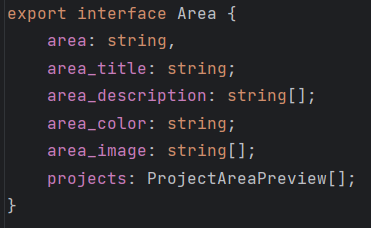
\includegraphics[width=6cm]{images/API/Area.png} 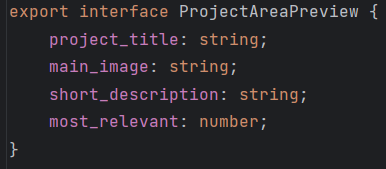
\includegraphics[width=6cm]{images/API/ProjectAreaPreview.png}
        \item StatusCode = 500 $\rightarrow$ StatusMessage = "Error form areas get"
        \item StatusCode = 404 $\rightarrow$ StatusMessage = "Not found"
    \end{itemize} 
\end{itemize}

\paragraph{/api/areas/\$area\_title}
\begin{itemize}
    \item \textbf{Request} \\ Type of request: GET \\ area\_title $\rightarrow$ parameter that corresponds to the area's key in the DB 
    \item \textbf{Response} \begin{itemize}
        \item StatusCode = 200 $\rightarrow$ The response contains an Area object (defined as below) \\ \\
            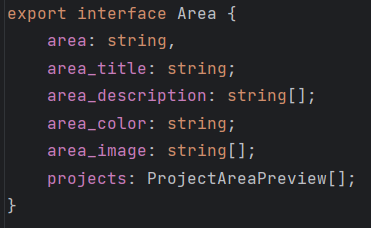
\includegraphics[width=6cm]{images/API/Area.png} 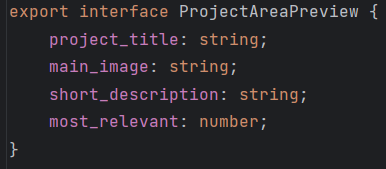
\includegraphics[width=6cm]{images/API/ProjectAreaPreview.png}
        \item StatusCode = 500 $\rightarrow$ StatusMessage = "Error form area\_id get"
        \item StatusCode = 404 $\rightarrow$ StatusMessage = "Not found"
    \end{itemize} 
\end{itemize}

\paragraph{/api/projects}
\begin{itemize}
    \item \textbf{Request} \\ Type of request: GET \\ No params 
    \item \textbf{Response} \begin{itemize}
        \item StatusCode = 200 $\rightarrow$ The response contains an array of Project object that corresponds to the info in the areas table in the database (the Project object is defined below)\\ \\
            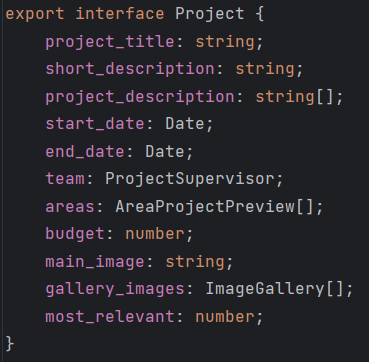
\includegraphics[width=6cm]{images/API/Project.png} 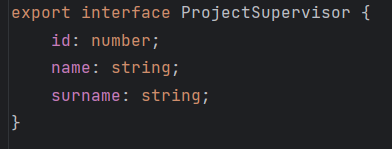
\includegraphics[width=6cm]{images/API/ProjectSuperv.png}  \\ 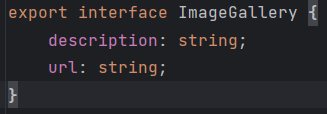
\includegraphics[width=6cm]{images/API/ImageGallery.png} 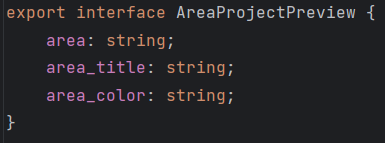
\includegraphics[width=6cm]{images/API/AreaPreview.png}
        \item StatusCode = 500 $\rightarrow$ StatusMessage = "Error form projects get"
        \item StatusCode = 404 $\rightarrow$ StatusMessage = "Not found"
    \end{itemize} 
\end{itemize}


\paragraph{/api/projects/\$project\_title}
\begin{itemize}
    \item \textbf{Request} \\ Type of request: GET \\ project\_title $\rightarrow$ parameter that corresponds to the project's key in the DB 
    \item \textbf{Response} \begin{itemize}
        \item StatusCode = 200 $\rightarrow$ The response contains an Project object (defined as below) \\ \\
            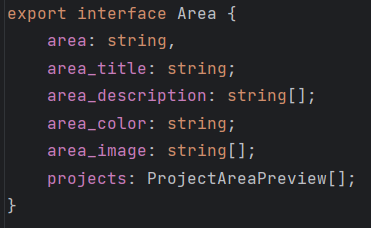
\includegraphics[width=6cm]{images/API/Area.png} 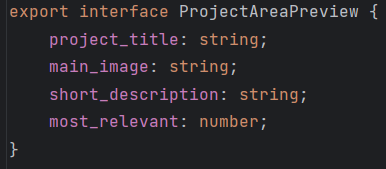
\includegraphics[width=6cm]{images/API/ProjectAreaPreview.png}
        \item StatusCode = 500 $\rightarrow$ StatusMessage = "Error form project\_title get"
        \item StatusCode = 404 $\rightarrow$ StatusMessage = "Not found"
    \end{itemize} 
\end{itemize}

\paragraph{/api/team}
\begin{itemize}
    \item \textbf{Request} \\ Type of request: GET \\ No params 
    \item \textbf{Response} \begin{itemize}
        \item StatusCode = 200 $\rightarrow$ The response contains an array of Person object that corresponds to the info in the areas table in the database (the Person object is defined below)\\ \\
            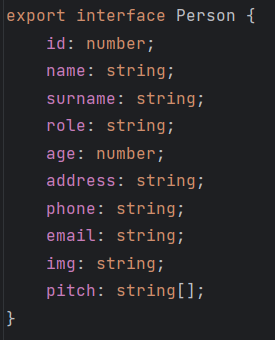
\includegraphics[width=6cm]{images/API/Person.png}
        \item StatusCode = 500 $\rightarrow$ StatusMessage = "Error from people get"
        \item StatusCode = 404 $\rightarrow$ StatusMessage = "Not found"
    \end{itemize} 
\end{itemize}

\paragraph{/api/team/\$surname\_name}
\begin{itemize}
    \item \textbf{Request} \\ Type of request: GET \\ surname\_name $\rightarrow$ parameter that corresponds to the person name and surname in the DB 
    \item \textbf{Response} \begin{itemize}
        \item StatusCode = 200 $\rightarrow$ The response contains  a Person object (defined as below) \\ \\
            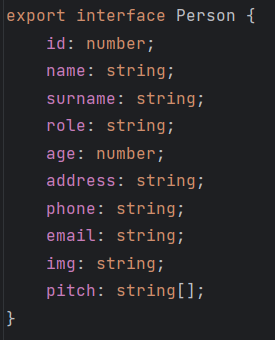
\includegraphics[width=6cm]{images/API/Person.png}
        \item StatusCode = 500 $\rightarrow$ StatusMessage = "Error from person get"
        \item StatusCode = 404 $\rightarrow$ StatusMessage = "Not found"
    \end{itemize} 
\end{itemize}

\paragraph{/api/team/\$surname\_name/projects}
\begin{itemize}
    \item \textbf{Request} \\ Type of request: GET \\ surname\_name $\rightarrow$ parameter that corresponds to the person name and surname in the DB  
    \item \textbf{Response} \begin{itemize}
        \item StatusCode = 200 $\rightarrow$ The response contains an array of Project object that corresponds to the info in the project table in the database (the Project object is defined below)\\ \\
            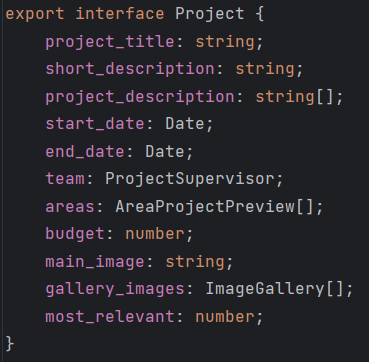
\includegraphics[width=6cm]{images/API/Project.png} 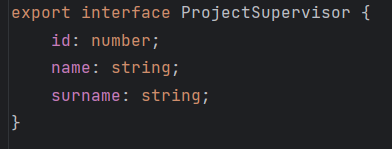
\includegraphics[width=6cm]{images/API/ProjectSuperv.png} \\ 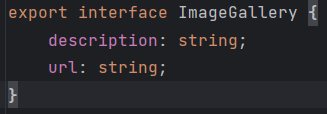
\includegraphics[width=6cm]{images/API/ImageGallery.png} 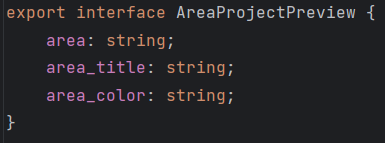
\includegraphics[width=6cm]{images/API/AreaPreview.png}
        \item StatusCode = 500 $\rightarrow$ StatusMessage = "Error from person-projects get"
        \item StatusCode = 404 $\rightarrow$ StatusMessage = "Not found"
    \end{itemize} 
\end{itemize}

\paragraph{/api/about\_us}
\begin{itemize}
    \item \textbf{Request} \\ Type of request: GET \\ No params 
    \item \textbf{Response} \begin{itemize}
        \item StatusCode = 200 $\rightarrow$ The response contains an array of AboutUs object that corresponds to the info in the about\_us table in the database (the AboutUs object is defined below) \\ \\
            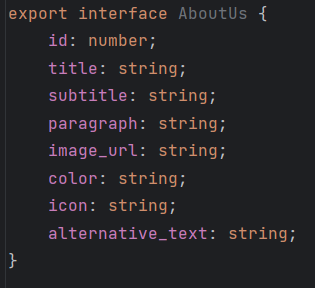
\includegraphics[width=6cm]{images/API/About_us.png}
        \item StatusCode = 500 $\rightarrow$ StatusMessage = "Error form about\_us get"
        \item StatusCode = 404 $\rightarrow$ StatusMessage = "Not found"
    \end{itemize} 
\end{itemize}

\paragraph{/api/contact\_us/pp\_form}
\begin{itemize}
    \item \textbf{Request} \\ Type of request: POST \\ Body:The body contains an object of a PPForm (defined as below) \\ \\
            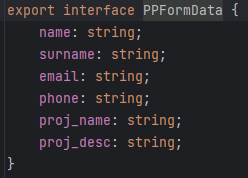
\includegraphics[width=6cm]{images/API/PPForm.png}
    \item \textbf{Response} \begin{itemize}
        \item StatusCode = 200 $\rightarrow$ StatusMessage = "OK"
        \item StatusCode = 500 $\rightarrow$ StatusMessage = "Invalid form"
    \end{itemize} 
\end{itemize}

\paragraph{/api/contact\_us/wwu\_form}
\begin{itemize}
    \item \textbf{Request} \\ Type of request: POST \\ Body:The body contains an object of a WWUForm (defined as below) \\ \\
            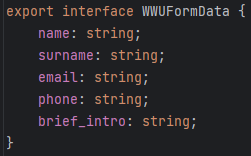
\includegraphics[width=6cm]{images/API/WWUForm.png}
    \item \textbf{Response} \begin{itemize}
        \item StatusCode = 200 $\rightarrow$ StatusMessage = "OK"
        \item StatusCode = 500 $\rightarrow$ StatusMessage = "Invalid form"
    \end{itemize} 
\end{itemize}

\subsection{List of Components implemented}
\begin{itemize}
    \item AreaSection: \\
        Area Section is a component used in the all areas display. It main purpose is to retrieve from the Database all the useful information regarding the area and show it on screen dynamically.
        For each area present it displays an image width full based on the screen visualizing it and in the center the Name of the area and the color associated with it. The color is useful to identify the area and will be reused later on, in the projects list as a tag.
    \item ProjectInfo: \\
        Project info is the component that shows all the useful information about a project, referring to Supervisor, Budget, Start Date, End Date and Related Areas. This is shown on the right part of the screen, next to the project description, that is handled by another component. The  becomes hidden behind a drop-down menu when the screen is resized under a certain dimension.
    \item ProjectInfoRow: \\
        This is a subcomponent used by ProjectInfo, its purpose is display each single row composed by an SVG, a short description and the belonging class.
    \item ProjectByArea: \\
        Here, an area and its relative projects are composed to be later shown. A single area, with its relative color, is displayed and has all its own project listed.
        The ProjectPreview component is reused to show the list of all available project belonging to that specific area, obviously, project belonging to multiple areas are displayed once each area.
        In order not to be too cumbersome, the projects could be hidden by clicking on the arrow next to the area name, so that those project that does not complain to the interest of the user could be avoided, making the page more readable and easier to navigate through.
    \item About Us: \\
        The About us section is meant to explain who we are and let the user familiarize with our work through multiple section, from a simple explanation about our company to which are our investment focus. Each section is characterized by the title, a color, an image, a little SVG on the left that is placed always besides its section and a description. All this is retrieved from the database and dynamically shown in the page.
    \item BackButton: \\
        Component that implements a button useful to go back to the area or project that the user was visualizing before. In the case of a small size screen it is a simple SVG circle with a left pointing arrow in the top-left corner of the screen, but it can be enriched with a label on bigger size screens.
    \item Dialog: \\
        This is a HTML dialog component that can ask the user a question and can redirect to a different website (Google Maps for locations) or contact someone (calling a phone number or emailing). In order to achieve this different goals, a function has to be passed to the component that will be triggered when the user confirms the action.
    \item Footer: \\
        The footer is a flex component with a left side composed of the Logo to be coherent with the header disposition (slightly bigger that the one on the top) and on the right useful links to orientate in the Website. Next, an horizontal line separates these components from other contact info like our group name on the left and link to socials like Facebook, Instagram, Github and Discord on the right.
        The disposition changes as soon as the screen reaches a dimension lower than 640px the flex direction changes from row to col with logo and useful link moving to the center, in order to be more appealing on a smartphone.
    \item FormSentDialogBox: \\
        This is the component used to show a positive response after a project is submitted and confirm that the request was sent.
    \item Header: \\
        The header component is a reusable items composed of a screen-wide div with the Logo on the left and a flex component on the right. The right part consist of all the label useful to reach the main pages of the Webapp like Areas, Projects, various form to contact the team and also a button to switch from dark to light mode. 
        Since the header has many label, in order to have a responsive and a good looking design as soon as the the screen reaches a width lower than 1024 pixels, the right part of the header became hidden and a burger-menu icon appears.\\
        This button allows the menu to be showed when clicked and keep the design clean and responsive even on lower screen dimensions.
    \item InfoBox: \\
        This component is the responsible for the displaying of the Company info like address, company phone, location and so on. All the information are linked to an app that can handle the request like, clicking on the address the Dialog component is invoked to inform the user that another tab with the Google Maps Display of the Company location.
    \item ProjectPreview: \\
        This component is widely used. The main purpose is to display a single project with its main image, a blurred part on the bottom containing the name of the project and eventually a short description and a set of tags depending on the areas it belongs.
        Is used in a single area to show projects relative to that specific area, obviously here the tag is omitted since is easy to retrieve the area in which the user currently is. \\
        Is used to show all the projects available in the Projects tab and also inside a member page to display the projects that member has taken part into. 
    \item ProposeProject: \\
        ProposeProject is the component responsible for showing all the fields needed to be filled in order to propose a project to StartMeUp. Is also responsible for all the assertion on the Name, e-mail address format constraint, phone number and so on.
    \item WorkWithUs: \\
        This last component is used to compose a work request proposal, where users can introduce themselves, leave all the contact details and even submit a resumé. This form as up above re-utilizes the dialog component in order to prevent mistake while compiling or sending.
\end{itemize}

\subsection{Extra components used}
\begin{itemize}
    \item Supabase, database used for retrieving information
    \item Vercel, platform for frontend developing and static websites
    \item Nuxt, web framework of the Next.js family
    \item Tailwind, CSS framework with packed and customizable classes
    \item Vuetify, framework used only to implement the timeline in the "About Us" page
\end{itemize}

\subsection{Extra functionalities}
\begin{itemize}
    \item A switch that changes from light to dark mode and viceversa, also the starting mode is based on the favourite theme of the browser.
    \item The \emph{dialog} helps the user to visually see that he/she is leaving the website in order to reach external links or contact a person.
    \item The \emph{details} HTML element is very useful because, when the screen width is small, long text paragraph will be reduced into smaller box that could be expanded on click. This helped us to keep the same design over a plethora of different screen sizes.
\end{itemize}

\subsection{Accessibility features}
All the important buttons and items have been marked with labels and title so that a text-2-speech software would allow a person to interact with the website in the correct way. Also the images have an alternative text that helps both for accessibility purpose and having a placeholder whether the picture cannot be or (in case of slow connection) is not already downloaded from the database. 

\section{Reference}
\begin{itemize}
    \item GitHub Repo: \url{https://github.com/stefanofossati/hypermedia-website}
    \item Website: \url{https://hypermedia-website.vercel.app/} \\ \url{https://hypermedia-website-stefanofossati.vercel.app/}
\end{itemize}

%%%%
\end{document}